% Adapted from UH Manoa theme by:
% UH Manoa presentation theme for beamer
% Jeff Delmerico <jeffdelmerico@gmail.com> 2012
% https://github.com/jeffdelmerico/UH_Beamer_Theme.git


\documentclass{beamer}
%\documentclass[handout]{beamer}
\usetheme{PD}

\usepackage[absolute,overlay]{textpos}
\usepackage{helvet}
\usepackage{tikz}
\usepackage{listings,lstautogobble}
\usetikzlibrary{tikzmark,fit}

\title{Ensuring Information Security \newline by Using Haskell Advanced Type System}
\subtitle{}
\author{Matteo Di Pirro}
\date{February 16th, 2017}
\institute{University of Padova}

\lstset{
	autogobble=true
}

\begin{document}

\newcommand{\turnOffNumbers}{true} %hide frame numbers in footer

\begin{frame}[noframenumbering]
\titlepage
\end{frame}

\let\turnOffNumbers\empty
\begin{frame}
	\frametitle{Outline}
	\tableofcontents
\end{frame}

\section{Software security}
\begin{frame}
\frametitle{What's Software Security?}
\begin{itemize}
	\item \textbf{Any} compromise to integrity, authentication and availability makes a software \textbf{unsecure}
	\item<2->{It is almost impossible to see how modern complex software can be abused}
\end{itemize}
\only<3->{
	\vspace{1em}
	\begin{center}
	\textit{"Program testing can be used to show the presence of bugs, but never to show their absence!"}
	\end{center}
	\textit{\hfill Edsger W. Dijkstra \\ \hfill Notes On Structured Programming}
}
\end{frame}
\begin{frame}{Language-based Security}
	\vspace{-2.5cm}
	\begin{textblock*}{2cm}(9cm,5cm)
		
\includegraphics[scale=0.15]{jif-logo}
	\end{textblock*}
	\begin{textblock*}{10cm}(2cm,5cm)
		\only<2->{$\rightarrow$ \textbf{New} languages from scratch} 
		\vspace{1cm}
		
		\only<3>{$\rightarrow$ \textbf{Simple} lightweight libraries}
	\end{textblock*}
	\begin{itemize}
		\item Language-based security is a useful complement to traditional security mechanisms
		\item Security-typed languages can rule out programs containing potential information leaks or integrity violations
	\end{itemize}
\end{frame}

\section{Haskell Modules}
	\subsection{Unsecure}
	\begin{frame}[fragile,containsverbatim]{The Unsecure module}
%\vspace{-1.5cm}
\begin{itemize}
	\item<1-> Ensures an input value will be validated before its use
	\item<1-> Is defined as a pair (Validation Functions, input value)
\end{itemize}	
\begin{center}
\vspace{1.5cm}
\begin{lstlisting}[basicstyle=\fontsize{9}{11}\ttfamily]
getSafeString :: Int -> IO (Unsecure String Bool)
getSafeString n = do l <- getLine
                     return $ upure [(\s -> length s <= n)]
\end{lstlisting}
\end{center}
\begin{tikzpicture}[remember picture,overlay]
\node<2->[white,font=\fontsize{0.4cm}{0.5cm}\selectfont](p) at (6,3.4) {Unsecure box};
\draw<2-> [->,white,line width=1pt] (6,2.2) -- (p);

\node<3->[white,font=\fontsize{0.4cm}{0.5cm}\selectfont](q) at (9,3.6) {Error type};
\draw<3-> [->,white,line width=1pt] (9,2.2) -- (q);

\node<4->[white,font=\fontsize{0.4cm}{0.5cm}\selectfont](r) at (8.8,0) {List of String $\rightarrow$ Bool functions};
\draw<4-> [->,white,line width=1pt] (8.8,1) -- (r);
\end{tikzpicture}
\end{frame}
	\subsection{SecureFlow}
	\begin{frame}{The SecureFlow module \newline Non-inference}
\begin{itemize}
	\item Inspired to the Lattice-Based Access Control
	\item Ensures non-inference among data
	\item Subjects may have different security levels at different times
\end{itemize}
\begin{figure}
	\centering
\includegraphics[scale=0.35]{informationflow}
\end{figure}
\end{frame}

	\begin{frame}{The SecureFlow module \newline Declassification}
	\vspace{-3cm}
	\begin{itemize}
		\item Declassification is a controlled way to leak \\information
	\end{itemize}
	\begin{textblock*}{2cm}(10.5cm,1.7cm)
		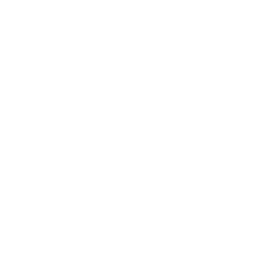
\includegraphics[scale=0.2]{hatch}
	\end{textblock*}
	\begin{tikzpicture}[remember picture,overlay]
	\node<2->[white,font=\fontsize{0.4cm}{0.5cm}\selectfont] at (1.8,-0.5) {Credential DB};
	\node<2->[white,font=\fontsize{0.4cm}{0.5cm}\selectfont] at (1.9,-1) {(Private)};
		
	\node<3->[white,font=\fontsize{0.4cm}{0.5cm}\selectfont] at (8.5,-0.5) {Public ticket};
	\node<3->[white,font=\fontsize{0.4cm}{0.5cm}\ttfamily\selectfont] at (8.5,-1) {open public credentials};
	\draw<3-> [->,white,line width=1pt] (6.5,-0.75) -- (3.3,-0.75);
	
	\node<4->[white,font=\fontsize{0.25cm}{0.5cm}\selectfont] at (5,-0.5) {Compilation error};
	
	\node<5->[white,font=\fontsize{0.4cm}{0.5cm}\selectfont] at (7.5,-3) {Declassification function};
	\node<5->[white,font=\fontsize{0.4cm}{0.5cm}\selectfont] at (7.5,-3.5) {Private $\rightarrow$ Public};
	\node<5->[white,font=\fontsize{0.4cm}{0.5cm}\ttfamily\selectfont] at (7.5,-4) {declassifyWith \textit{HatchFunction} credentials};
	\draw<5-> [->,white,line width=1pt] (6.5,-2.8) -- (3.3,-0.75);	

	\node<6->[white,font=\fontsize{0.25cm}{0.5cm}\selectfont] at (4,-2) {Access allowed};
	\end{tikzpicture}
\end{frame}
	
	\subsection{SecureComputation}
	\begin{frame}[fragile]{The SecureComputation module}
	\begin{itemize}
		\item Ensures compile time taint analysis
		\item Operations on sensitive data may be allowed only with untainted values
	\end{itemize}
	\hspace{-2cm}
	\begin{lstlisting}[basicstyle=\fontsize{9}{9}\ttfamily]
	getUnpureVal :: IO (SecureComputation T String)
	getUnpureVal = do n <- getLine
	                  return $ spure n
	\end{lstlisting}
	\begin{onlyenv}<3->
		\begin{lstlisting}[basicstyle=\fontsize{9}{9}\ttfamily]
		fun :: SC P Model -> SC P String -> SC P Model
		\end{lstlisting}
	\end{onlyenv}
	\begin{tikzpicture}[remember picture,overlay]
	\node<2>[draw,minimum size=0.5cm,line width=1pt,white,circle,label=above:{\color{white}Tainted}] at (7.65,1.4) {};
	
	\node<4>[draw,minimum size=0.5cm,line width=1pt,white,circle,label=below:{\color{white}Pure value required}] at (4.9,0.8) {};
	\end{tikzpicture}
	\begin{itemize}
		\item<5> \textbf{Compilation error} if \texttt{getUnpureVal} is used as a \texttt{fun} parameter
	\end{itemize}
\end{frame}
	
\section{Conclusions}
\begin{frame}{Conclusions}
	\begin{itemize}
		\item \textbf{Contribution}
		\begin{itemize}
			\item Three new types for ensuring three different properties
			\item Static and dynamic checking
			\item Based on widespread functional programming concepts
			\item Supposed to be used in small parts of the entire software
		\end{itemize}
		\vspace{1.5cm}
		\item<2-> \textbf{Limitations}
			\begin{itemize}
				\item New I/O functions required for introducing new types
				\item Type constraints in \texttt{Unsecure} and \texttt{SecureComputation}
				\item No relation between \texttt{Unsecure} and \texttt{SecureComputation}
			\end{itemize}
	\end{itemize}
\end{frame}
	
\appendix
\makethanks
\renewcommand{\turnOffNumbers}{true} %hide frame numbers in footer
% extra slides
\end{document}
